% =============================================================
%  CS102-F26 Digital Design and Computer Architecture I
%  Lecture 11 -- The Clock and Latches (Unit 11)
%  Follows Sections 5.2, 5.3, 5.3.1 and 5.3.2 of
%  A Student's Computer Architecture Book I.
%
%  Build the slides and the print handout:  npm run materials -- lecture-11
% =============================================================
\makeatletter
\def\input@path{{templates/latex/}{../}}
\makeatother

\documentclass[10pt]{wosm-slides}
\usepackage{cs102-lectures}[2026/10/20]

\title[Lecture 11 \textperiodcentered\ The Clock and Latches]{The Clock and Latches}
\subtitle{Lecture 11: the clock, memory, the SR latch and the D latch}

% ---------- Helpers for this lecture --------------------------
% Wider input spacing than the course default, so input labels fit.
\tikzset{gates/.append style={
  and gate/.append style={logic gate input sep=0.36cm},
  nand gate/.append style={logic gate input sep=0.36cm}}}
\tikzset{block/.style={draw=wosm-text, line width=0.6pt, minimum width=1.4cm,
  minimum height=1.2cm, font=\scriptsize, align=center}}

% The SR latch of the book: two NAND gates, inputs inverted.
% \srlatch{<label of S>}{<label of R>}
\newcommand*\srlatch[2]{%
  \begin{tikzpicture}[gates]
    \node[nand gate, inputs={in}] (g1) at (2,0.8) {};
    \node[nand gate, inputs={ni}] (g2) at (2,-0.8) {};
    \draw[wire] (g1.input 1) -- ++(-1.2,0) node[left] {#1};
    \draw[wire] (g2.input 2) -- ++(-1.2,0) node[left] {#2};
    \draw[wire] (g1.output) -- ++(0.9,0) node[right] {$Q$};
    \draw[wire] (g2.output) -- ++(0.9,0) node[right] {$\overline{Q}$};
    \coordinate (q) at ($(g1.output)+(0.4,0)$);
    \coordinate (qb) at ($(g2.output)+(0.4,0)$);
    \draw[wire] (q) -- ++(0,-0.55) -| ($(g2.input 1)+(-0.3,0)$) -- (g2.input 1);
    \draw[wire] (qb) -- ++(0,0.55) -| ($(g1.input 2)+(-0.6,0)$) -- (g1.input 2);
    \fill[wosm-text] (q) circle (1.5pt);
    \fill[wosm-text] (qb) circle (1.5pt);
  \end{tikzpicture}}

% =============================================================
\begin{document}

\maketitle

\begin{frame}{Today}
  \tableofcontents
\end{frame}

% =============================================================
\section{The clock}

\begin{frame}{A clock for a computer}
  A clock orchestrates all of us at once. Inside a computer, a clock orchestrates
  all the parts. Its face has only two numbers: 0 and 1.

  \medskip
  \begin{center}
    \begin{tikzpicture}[x=0.55cm]
      \foreach \t in {2,6,10,14} {\timingedge{\t}{1}}
      \timingwave{0}{clock}{0,0,1,1,0,0,1,1,0,0,1,1,0,0,1,1,0,0}
      \draw[wosm-accent, line width=0.5pt, {Stealth[length=3pt]}-{Stealth[length=3pt]}]
        (2,-0.3) -- node[below, font=\scriptsize] {period $T$} (6,-0.3);
      \node[above, font=\tiny, text=wosm-muted] at (10,0.32) {rising edge};
      \node[above, font=\tiny, text=wosm-muted] at (12.6,0.32) {falling edge};
    \end{tikzpicture}
  \end{center}

  \begin{itemize}
    \item The \alert{period} $T$ is the time for one full cycle; the
      \alert{frequency} is $f = 1/T$, in hertz (cycles per second).
    \item A \emph{rising} edge goes from 0 to 1, a \emph{falling} edge from 1 to 0.
      The \emph{duty cycle} is the share of the period spent at 1, usually 50\%.
  \end{itemize}
\end{frame}

\begin{frame}{Periods and frequencies}
  \begin{center}
    \begin{tabular}{@{}lll@{}}
      \toprule
      Period $T$ & Frequency $f = 1/T$ & \\
      \midrule
      10\,\textmu s & 100\,kHz & the clock in the book's Figure 5.7 \\
      5\,ns & 200\,MHz & the speed limit of Lecture 09's example circuit \\
      0.33\,ns & 3\,GHz & a typical processor today \\
      \bottomrule
    \end{tabular}
  \end{center}

  \bigskip
  \begin{remark}
    Every part of a synchronous circuit does its work between two ticks. So the clock
    can tick only as fast as the slowest part allows: a period shorter than its
    propagation delay gives wrong results \unitref{14}.
  \end{remark}
\end{frame}

\begin{frame}{Making a clock}
  \begin{columns}[c, totalwidth=\textwidth]
    \column{0.42\textwidth}
      \centering
      \begin{tikzpicture}[gates]
        \node[not gate] (n1) at (0,0) {};
        \node[not gate] (n2) at (1.3,0) {};
        \node[not gate] (n3) at (2.6,0) {};
        \draw[wire] (n1.output) -- (n2.input) (n2.output) -- (n3.input);
        \draw[wire] (n3.output) -- ++(0.3,0) coordinate (o) -- ++(0,-0.6) -| ($(n1.input)+(-0.3,0)$)
          -- (n1.input);
        \fill[wosm-text] (o) circle (1.5pt);
        \draw[wire] (o) -- ++(0.4,0) node[right] {clock};
      \end{tikzpicture}\par\medskip
      \wosmlabel{a ring of three NOT gates}
    \column{0.54\textwidth}
      \begin{itemize}
        \item The book's clock is one NOT gate whose output feeds its own input: the
          output can never settle, so it keeps flipping.
        \item In a real circuit we use a ring of an \alert{odd} number $n \ge 3$ of NOT
          gates. Each half period takes $n$ gate delays, so $T = 2\,n\,t_{pd}$.
        \item Computers take their clock from a quartz crystal, and multiply its
          frequency on the chip.
      \end{itemize}
  \end{columns}

  \bigskip
  \wosmlabel{With an even number of NOT gates the ring settles and never flips:
  remember this for the next slide.}
\end{frame}

% =============================================================
\section{Memory}

\begin{frame}{What is memory?}
  \begin{columns}[c, totalwidth=\textwidth]
    \column{0.36\textwidth}
      \centering
      \begin{tikzpicture}[gates]
        \node[not gate] (n1) at (0,0) {};
        \node[not gate] (n2) at (1.4,0) {};
        \draw[wire] (n1.output) -- (n2.input);
        \draw[wire] (n2.output) -- ++(0.3,0) coordinate (o) -- ++(0,-0.6) -| ($(n1.input)+(-0.3,0)$)
          -- (n1.input);
        \fill[wosm-text] (o) circle (1.5pt);
        \draw[wire] (o) -- ++(0.35,0) node[right] {$Q$};
      \end{tikzpicture}\par\medskip
      \wosmlabel{two NOT gates in a ring}
    \column{0.6\textwidth}
      \begin{itemize}
        \item Memory is something that persists while everything around it changes.
        \item Two NOT gates in a ring keep their value forever. But they keep whatever
          they started with: there is no way to put a value in.
        \item Better: memory is something that is \alert{updated} in certain
          situations and \alert{kept} in all others.
      \end{itemize}
  \end{columns}
\end{frame}

\begin{frame}{A memory with two inputs}
  Give the circuit two inputs, (memorize-1, memorize-0):
  \begin{itemize}
    \item (1, 0): remember 1; \quad (0, 1): remember 0; \quad (0, 0): keep what is
      stored;
    \item (1, 1) makes no sense: one bit cannot remember 1 and 0 at once.
  \end{itemize}

  \medskip
  \begin{center}
    \begin{tabular}{@{}l|ccccc@{}}
      Time step & 0 & 1 & 2 & 3 & 4 \\
      \midrule
      Input & (1, 0) & (0, 0) & (0, 0) & (0, 1) & (0, 0) \\
      Output & 1 & 1 & 1 & 0 & 0 \\
    \end{tabular}
  \end{center}

  \medskip
  \begin{remark}[It is the mystic box]
    Lecture 10's box with \emph{On} as memorize-1, \emph{Off} as memorize-0, and green
    as 1. We found $Q^{+} = \mathit{On} + \mathit{Off}'\,Q$.
  \end{remark}
\end{frame}

\begin{frame}{Set, reset, hold}
  \begin{columns}[c, totalwidth=\textwidth]
    \column{0.42\textwidth}
      \centering
      \begin{tabular}{@{}cc|cc@{}}
        $S$ & $R$ & $Q_{t+1}$ & $Q'_{t+1}$ \\
        \midrule
        0 & 0 & $Q_t$ & $Q'_t$ \\
        0 & 1 & 0 & 1 \\
        1 & 0 & 1 & 0 \\
        1 & 1 & \multicolumn{2}{c}{not allowed} \\
      \end{tabular}\par\medskip
      \wosmlabel{S: set (memorize-1); R: reset (memorize-0)}
    \column{0.54\textwidth}
      \begin{itemize}
        \item The output is also given as a complement pair, $Q$ and $Q'$.
        \item Input (0, 0) gives 0 at some times and 1 at others, depending on the past.
          So no combinational circuit can do this: the circuit must be
          \alert{sequential}.
      \end{itemize}
  \end{columns}
\end{frame}

% =============================================================
\section{The SR latch}

\begin{frame}{The SR latch}
  \begin{columns}[c, totalwidth=\textwidth]
    \column{0.5\textwidth}
      \centering
      \srlatch{$S$}{$R$}
    \column{0.46\textwidth}
      \begin{itemize}
        \item Two NAND gates, each fed by the other's output. The bubbles on $S$ and
          $R$ are NOT gates.
        \item The top gate outputs what is stored, $Q$; the bottom one its opposite,
          $\overline{Q}$:
          \[ \begin{aligned} Q &= \mathrm{NAND}(S', \overline{Q}) \\
             \overline{Q} &= \mathrm{NAND}(R', Q) \end{aligned} \]
      \end{itemize}
  \end{columns}

  \medskip
  \wosmlabel{A NAND outputs 0 only when both inputs are 1. So a 0 on either input forces
  its output to 1.}
\end{frame}

\begin{frame}{Setting and holding}
  \begin{columns}[T, totalwidth=\textwidth]
    \column{0.47\textwidth}
      \textbf{Set:} $S = 1$, $R = 0$, stored $Q = 0$.
      \begin{enumerate}
        \item $S' = 0$, so the top NAND outputs $Q = 1$.
        \item Now the bottom NAND sees $R' = 1$ and $Q = 1$: $\overline{Q} = 0$.
        \item The top NAND sees $S' = 0$ and $\overline{Q} = 0$: $Q$ stays 1. Stable.
      \end{enumerate}
    \column{0.47\textwidth}
      \textbf{Hold:} then $S = R = 0$, stored $Q = 1$.
      \begin{enumerate}
        \item Both NANDs now see a 1 from their inverted input.
        \item Top: $\mathrm{NAND}(1, \overline{Q} = 0) = 1$. Bottom:
          $\mathrm{NAND}(1, Q = 1) = 0$.
        \item Nothing changes: the latch keeps $Q = 1$.
      \end{enumerate}
  \end{columns}

  \bigskip
  \begin{remark}
    With $S = R = 0$ each gate passes on the complement of the other's output: the
    latch is the two-NOT ring of the last section. $S$ and $R$ are the way to write it.
  \end{remark}
\end{frame}

\begin{frame}{The full truth table}
  \begin{center}
    \small
    \begin{tabular}{@{}ccc|cc|l@{}}
      $S$ & $R$ & $Q_t$ & $Q_{t+1}$ & $\overline{Q}_{t+1}$ & \\
      \midrule
      0 & 0 & 0 & 0 & 1 & hold \\
      0 & 0 & 1 & 1 & 0 & hold \\
      0 & 1 & 0 & 0 & 1 & reset \\
      0 & 1 & 1 & 0 & 1 & reset \\
      1 & 0 & 0 & 1 & 0 & set \\
      1 & 0 & 1 & 1 & 0 & set \\
      1 & 1 & 0 & \alert{1} & \alert{1} & not valid: $Q = \overline{Q}$ \\
      1 & 1 & 1 & \alert{1} & \alert{1} & not valid: $Q = \overline{Q}$ \\
    \end{tabular}
  \end{center}

  \medskip
  Check each row yourself by pushing the inputs through the circuit, as in the book.
\end{frame}

\begin{frame}{The forbidden input}
  With $S = R = 1$ both outputs are 1. That alone is wrong, but worse comes when both
  inputs go back to 0:

  \medskip
  \begin{center}
    \begin{tabular}{@{}ll@{}}
      \toprule
      Released first & Result \\
      \midrule
      $S$ & $R$ is still 1 for a moment: the latch resets, $Q = 0$ \\
      $R$ & $S$ is still 1 for a moment: the latch sets, $Q = 1$ \\
      both at exactly the same time & no input wins: $Q$ may flip back and forth \\
      \bottomrule
    \end{tabular}
  \end{center}

  \medskip
  \begin{itemize}
    \item The input released \alert{last} wins, and which one that is depends on tiny
      differences in timing.
    \item Stuck between 0 and 1 for a while is called \alert{metastability}.
    \item The rule: never apply $S = R = 1$.
  \end{itemize}
  \wosmlabel{Built from two NOR gates instead, the latch works the same, except that
  $S = R = 1$ makes both outputs 0.}
\end{frame}

% =============================================================
\section{The D latch}

\begin{frame}{The D latch}
  \begin{columns}[c, totalwidth=\textwidth]
    \column{0.3\textwidth}
      \centering
      \begin{tabular}{@{}cc|c@{}}
        $D$ & $E$ & $Q_{t+1}$ \\
        \midrule
        0 & 0 & $Q_t$ \\
        1 & 0 & $Q_t$ \\
        0 & 1 & 0 \\
        1 & 1 & 1 \\
      \end{tabular}
    \column{0.66\textwidth}
      \begin{definition}[D latch]
        A \emph{D latch} has a data input $D$ and an enable input $E$. While $E = 1$
        it stores $D$; while $E = 0$ it keeps what it has.
      \end{definition}
  \end{columns}

  \bigskip
  \begin{itemize}
    \item While $E = 1$, the output follows $D$: the latch is \alert{transparent}.
    \item While $E = 0$ it is \alert{opaque}: $D$ can change freely, $Q$ does not.
  \end{itemize}
\end{frame}

\begin{frame}{From an SR latch to a D latch}
  \begin{columns}[c, totalwidth=\textwidth]
    \column{0.38\textwidth}
      \centering
      \begin{tabular}{@{}cc|cc|c@{}}
        $D$ & $E$ & $S$ & $R$ & $Q_{t+1}$ \\
        \midrule
        0 & 0 & 0 & 0 & $Q_t$ \\
        1 & 0 & 0 & 0 & $Q_t$ \\
        0 & 1 & 0 & 1 & 0 \\
        1 & 1 & 1 & 0 & 1 \\
      \end{tabular}\par\medskip
      $S = D E, \qquad R = D' E$
    \column{0.58\textwidth}
      \centering
      \begin{tikzpicture}[gates]
        \coordinate (left) at (0,0);
        \node[and gate, inputs=nn] (a1) at (2.9,0.6) {};
        \node[and gate, inputs=nn] (a2) at (2.9,-0.6) {};
        \node[block] (l) at (4.9,0) {SR\\latch};
        \node[not gate] (n) at ($(a2.input 1)+(-0.8,0)$) {};
        \node (d) at (a1.input 1 -| left) {$D$};
        \node (e) at (a2.input 2 -| left) {$E$};
        \draw[wire] (d) -- (a1.input 1);
        \draw[wire] (d -| 0.35,0) |- (n.input);
        \draw[wire] (n.output) -- (a2.input 1);
        \fill[wosm-text] (d -| 0.35,0) circle (1.5pt);
        \draw[wire] (e) -- (a2.input 2);
        \draw[wire] (e -| 0.6,0) |- (a1.input 2);
        \fill[wosm-text] (e -| 0.6,0) circle (1.5pt);
        \draw[wire] (a1.output) -- ++(0.3,0) |- ($(l.west)+(0,0.3)$)
          node[right, font=\tiny] {S};
        \draw[wire] (a2.output) -- ++(0.3,0) |- ($(l.west)+(0,-0.3)$)
          node[right, font=\tiny] {R};
        \draw[wire] (l.east) -- ++(0.4,0) node[right] {$Q$};
      \end{tikzpicture}
  \end{columns}

  \bigskip
  \begin{itemize}
    \item The book's view: put a small \enquote{interface} in front of the SR latch that
      turns $(D, E)$ into $(S, R)$.
    \item $S$ and $R$ can never both be 1, since $D$ and $D'$ never are: the D latch has
      \alert{no invalid inputs}.
  \end{itemize}
\end{frame}

\begin{frame}{The D latch in time}
  \begin{center}
    \begin{tikzpicture}[x=0.75cm]
      \foreach \t in {2,5,8,10} {\timingedge{\t}{3}}
      \timingwave{0}{$E$}{0,0,1,1,1,0,0,0,1,1,0,0}
      \timingwave{1}{$D$}{0,1,1,0,1,1,0,0,0,1,1,0}
      \timingwave{2}{$Q$}{0,0,1,0,1,1,1,1,0,1,1,1}
    \end{tikzpicture}
  \end{center}

  \begin{itemize}
    \item While $E = 1$, $Q$ copies every change of $D$, even several in a row.
    \item When $E$ falls, $Q$ keeps the last value of $D$: 1 after the first window,
      1 after the second.
    \item While $E = 0$, $D$ changes without effect.
  \end{itemize}
\end{frame}

\begin{frame}{The trouble with transparency}
  \begin{columns}[c, totalwidth=\textwidth]
    \column{0.4\textwidth}
      \centering
      \begin{tikzpicture}[gates]
        \pic (l) at (0,0) {dlatch};
        \node[not gate] (n) at (0.1,1.1) {};
        \draw[wire] (l-q) -- ++(0.35,0) coordinate (o) |- (n.output);
        \draw[wire] (n.input) -- ++(-0.5,0) |- (l-d);
        \fill[wosm-text] (o) circle (1.5pt);
        \draw[wire] (o) -- ++(0.4,0) node[right] {$Q$};
        \draw[wire] (l-e) -- ++(-0.6,0) node[left] {clock};
      \end{tikzpicture}
    \column{0.56\textwidth}
      \begin{itemize}
        \item We want a bit that flips once per clock tick: $D = Q'$, enabled by the
          clock.
        \item But while the clock is 1 the latch is transparent, and the loop is a ring
          oscillator: $Q$ flips again and again.
        \item We need a memory that changes only at the \alert{instant} of a clock
          edge.
      \end{itemize}
  \end{columns}

  \bigskip
  \begin{block}{Next lecture}
    The flip-flop: built from two D latches, it reacts to the clock edge, not to the
    clock level.
  \end{block}
\end{frame}

\begin{frame}{Try it}
  \begin{enumerate}
    \item What is the frequency of a clock with a period of 2\,ns?\par
      \uncover<2->{\small $f = 1 / 2\,\mathrm{ns} = 500$\,MHz.}
    \item A ring of 5 NOT gates, each with a delay of 20\,ps. What period, and what
      frequency?\par
      \uncover<3->{\small $T = 2 \times 5 \times 20\,\mathrm{ps} = 200$\,ps, so
      $f = 5$\,GHz.}
    \item An SR latch holds $Q = 1$. Apply $S = 0$, $R = 1$, then $S = R = 0$. What is
      $Q$?\par
      \uncover<4->{\small 0: the reset stores 0, and the hold keeps it.}
    \item A D latch has $E = 1$ while $D$ goes 0, 1, 0; then $E = 0$ and $D = 1$.
      What is $Q$ at the end?\par
      \uncover<5->{\small 0, the value of $D$ when $E$ fell.}
  \end{enumerate}
\end{frame}

% =============================================================
\section{Summary}

\begin{frame}{Summary}
  \begin{itemize}
    \item A clock is a signal that flips between 0 and 1 with period $T$ and frequency
      $f = 1/T$. A ring of an odd number of NOT gates makes one.
    \item Memory must be writable: update in some situations, hold in all others.
    \item The SR latch: set, reset, hold. $S = R = 1$ is not allowed, and releasing it
      can leave the latch metastable.
    \item The D latch: $Q$ follows $D$ while $E = 1$, and holds while $E = 0$. It has no
      invalid inputs.
    \item Transparency is a problem when a latch's output feeds back to its input:
      we need edge-triggered memory.
  \end{itemize}
\end{frame}

\begin{frame}{Before the next lecture}
  \begin{itemize}
    \item Read Sections~5.2, 5.3, 5.3.1 and 5.3.2 of the book.
    \item In Logisim-evolution, build the SR latch from NAND and NOT gates, and check
      every row of its truth table.
    \item Build a D latch on top of it, and drive $E$ from a clock. Watch $Q$ follow $D$
      while the clock is 1.
  \end{itemize}

  \begin{block}{Next lecture \unitref{12}}
    Flip-flops: the master--slave D flip-flop, asynchronous reset, and T and JK
    flip-flops.
  \end{block}
\end{frame}

\end{document}
